%% The bib stuff for this and chapter 2 is in the essay!

\chapter {Design Alternatives for Modern Web Applications}
\section{Introduction}
So far we have discussed the behavioral trends in modern web applications, and some common technologies that enables such applications. We saw that modern web applications are often very interactive with rich user interfaces, and that these web sites looks and performs like native desktop applications with graphical user interfaces. In addition there is often a requirement for a high number of simultaneous users, and a lot of data is being stored and manipulated. In this chapter, we look at the various technologies that are commonly used to design and build such interactive and scalable software applications. This concerns the application's \textbf{architecture}. The application's architecture describes the concepts of the application's structure, at different granularities. In this thesis, we will discuss architectures both seen at a high-level perspective, and also down to low-level source code perspectives.

As the behavioral requirements for web applications has increasingly changed the last years, so has the application's software architectures. The traditional web application has in the last decade followed a three-layered architecture where all the logic happens on the server. This is called a fat-server architecture, where HTML pages are rendered on the server and handed to the browser every time the client issues an Http request. Lately however, there has been an increasing interest in moving much of the applications logic to the client, and abandoning the server-side page rendering in favor for client-side page rendering for dynamic HTML content. This is called a thick client architecture. \footnote{The thick client architecture is not a new idea; thick client architectures has been around for many years, where programs are sent from the server and executed in the client. Often this would be online games, calculators, or other user-interactive applications. However, these applications depend on a specific program that is compiled and executed on the client, in other words, not traditional web pages that uses common browser-supported technologies.} Still however, a lot of applications follows the traditional approach, as many developers and application owners are skeptical to the fat-client model. This architecture implies heavy use of JavaScript, which has since its beginning had a lot of opposition, and there are still many browsers that does not fully support JavaScript behavior. 

The main purpose of this chapter is to outline the differences between the traditional web-app architecture, and modern web-app architecture. We will look at common trends and popular solutions in how developers often design and implement the respective architectural models. The first part of this chapter is divided into two main sections, one for each architecture. After this we will explain how these solutions have been deployed in the prototypes built for this thesis. For simplicity purposes, we will refer to the traditional approach as \textbf{Reference-model 1.0}, while the latter approach will be referred to as \textbf{Reference-model 2.0}. Hence, these two will be our reference models for software architectures that are aimed to build modern, interactive and scalable web apps. 

\section{Traditional Web Application Architecture}
Going back approximately 15 years, web applications where often built with CGI technology using tools like Perl and ColdFusion \cite{webstart} . With the CGI technology, a web server accepts URLs that are delegated to an appropriate CGI program. A process is started on the server, and the CGI program executes the given request, which results in an HTML page that is sent back to the client. This solution however, was not very scalable considering each request would trigger a new process on the server. Gradually, as the web got more users and the applications became more complex, new web framework technologies came along. Examples are PHP, J2EE, Ruby on Rails and Microsoft's .NET \cite{topframeworks}. For many years, developers have been building web applications with these technologies, where all of the application's business operations are executed on the server. This implies that the backend implementation has many responsibilities, and the front-end is simply a thin client that doesn't need to do much processing. This is only logical, as backend implementations runs on powerful web servers, and client devices has up until recent years not been able to perform demanding processing jobs. 

In an HTTP request, the backend application receives requests (often named an \textbf{action}) from a client which is handled by a \textbf{request handler}. The handler performs validation of the input data, executes the necessary business logic, and if necessary, manipulates the database. To be able to serve multiple simultaneous users, the application server often generates a separate thread for each incoming request. At the end of the handler's execution sequence, the application prepares an HTML page that it sends back to the client. The client tier refers to the front-end code that runs in the client's browser. It consists of an HTML and zero or more CSS files. The modern web application proposed in this thesis requires a lot of interactive behavior which is usually best solved with  JavaScript. Other popular alternatives to JavaScript are for example Flash, Microsoft Silverlight, or ActiveX. However, these all have in common that most browsers don't support them out of the box, meaning a plugin has to be downloaded and installed in order to use any one of them. Also, these technologies tend to provide their own graphical user interface, so that when they are integrated into the web app, they tend to look different then the web app's own "style". 

The HTML file contains just the necessary JavaScript code to enhance the user experience. The script code is either embedded in the HTML file inside \textit{script} tags, or it is referenced as external JavaScript files that must be fetched by the browser. The JavaScript code is often a collection of \textbf{event-handlers}, which are independent functions registered to be notified when a given event happens in the browser. Examples of events is when a mouse is clicked that will start an animation, the mouse is hovering over an image, a button is clicked that will open a small pop-up window, or some text is entered that needs quick validation. The event-handler will look at the current state of the web page, execute some necessary JavaScript routine, possibly making an Ajax request to the server to get some data, then manipulate the browser's DOM tree to update the page. Note that the JavaScript event handlers are only used for small-sized user events that needs quick results. User actions that leads to bigger changes, like URL- or form requests are not handled by JavaScript but are normal HTTP requests sent directly to the server, leading to a new HTML page sent back to the client. 

%When the browser receives the data from the server, it will do nothing more then simply display the %data, and not perform any additional business logic. This is a best-practise  usage scheme that is %recommended by most web developers \cite{separateBusiness}. and is referred to as a thin client %model.	 

% flash er n� bakt inn i chrome og ie 10.
% Flash og java er vanligvis brukt til multimedia shit



%%% Need form validation both on client side and server in case user has shut off client side JS. 
% He could submit invalid data, and abuse the server impl. We can have client side validation for efficiency reason in addition to it. 

%% Script tag in head blocks browser 
%% Script in bottom, can let page render so user sees stuff while page loads
%% Script tags blocks, therefore asynchronous module loading.
	
%The server maintains state for each user, most often by using an HTTP-session implementation. This %way, the first time the client uses the app, the server creates a session object that is used to %remember what the user has done.

%	The backend implementation in a \textit{web app}, is the code that runs
%on the server. This is often deployd
%	in an application server. The backend code is invoked by a web server
%application, that sits
%	and listens for incoming http connections. In the traditional approach,
%the user executes an
%	http request each time it triggers an html form, or requests a url
%either in the address bar or through
%	an html link tag. An html form is a component that wraps other input
%components like a button, textfield, date picker etc.
%	In other words, each time the user initiates an action, an http request
%is sent to the server. 
%	In this case, the server would respond with a complete html page that
%the browser renders so the user can see it on the screen. Also, it is not
%	the case that the server sends the whole web page in one http response
%packet. Each reference to other resources that are embedded in the html page (which
%could for instance be a movie reference, css style sheet reference, or javascript source file
%reference) are fetched in a separate http request. In some cases the response from
%the server could be an http redirect,
%	which is an instruction to tell the client to make a
%	request for a new page. This would in effect require a
%	(minimum) number of 4 client-server interactions! Considering that this
%process	is synchronous (because the client has to wait until the server has sent
%the html page back), it might lead to tedious waiting time for the client
%user.
%	
%	\subsubsection{Ajax}
%	Obviously, this interaction scheme is not always ideal for interactive
%web applications, especially if only a minor part of the web page is changed in
%the http request. Hence, having to send a complete html page each time the user
%performs an
%	action is in many cases a waste of network traffic. This has lead to
%another popular
%	client-server technology called Ajax \cite{ajx}. In this interaction
%scheme the browser
%	would only ask the server for a specific web resource. This could for
%instance be a blog
%	post or comment represented in a markup language like XML \cite{xml}.
%When the browser receives this resource
%	from the server, it would embed it into the already rendered web page.
%This process happens 
%	asynchronusly, and the web page is not refreshed upon completion. In
%result, there user wouldn't
%	have to wait for some data transfer to finish (since it happens
%asynchronously behind the scenes),
%	and the received data is much more fine-grained.
%	
%	\subsection{Client state}
%	Since http is stateless, the server has to maintain state between a
%given client's requests in order to avoid having to ask for user credentials all
%the time. 
%Now, there are a couple of ways to solve this, and it is usually implemented in
%web application frameworks.
%Some choose to put a unique id in cookies, and some choose to add an id to each url,
%or inside hidden fields in html forms. The most common choice however, is to use
%so-called html session objects. This is implemented as a token identifier that
%is stored either in a cookie or in the url (if cookies are not supported by the
%browser). This is called a session object, and is 
%included in every http request the user sends to the server. Hence, the server
%has to maintain a session
%object in memory for every user that is accessing the page at any given time. An
%example is given in figure \vref{fig:httpsession}. The session object is often used a cache for data object that the given user would access often. This avoids having to fetch the same data from the database needless times.
%
%\begin{figure}
%
%\fbox{\includegraphics[width=\textwidth,height=\textheight,keepaspectratio] 
%{images/httpsession.jpg}}
%\caption{A HTTP request with a seesion identifier in the cookie}
%\label{fig:httpsession}
%\end{figure} 

%\subsection{Server-side page rendering} 	
%	In dynamic web pages, when an http request comes in from the user,
%	the server has to have a way of dynamically updating the given html page
%	that is requested with new data. This might be data recently fetched from a database, or maybe some data
%	that is currently stored in the servers memory. The html page is often
%	generated on the server by using a so-called templating engine. This 
%	component will take as input a map of data variables, and a so-called
%	template file. The template file is a source file written in a domain
%	specific language. This language extends html with a set of predefined tags.
%	The tags represents basic programming concepts like variables, loops, and
%condition statements.
%	When the templating engine executes the rendering job, it 
%	transforms the template file and the data map into a complete html page
%	that it sends back to the client. 
	

	
\subsection{The Three-Layered Architecture}		
A classical way of separating concerns in a web application is to divide the whole system into three different software layers. This is called a three-layered architecture. There are some variations to how these layers are separated, but in this thesis, when we refer to the three-layered architecture, we follow the layering structure outlined by Brown et. al.\cite{brown} This architecture separates the system into a Presentation layer, domain layer, and a data source layer. These layers reside exclusively on the backend of the application. The front-end (e.g the code that runs on the client) has little responsibility in this architecture, as its only task is to display the result that is produced on the backend. The layers are designed to be very loose coupled. This is done by avoiding that a module in one layer depends on a concrete implementation in a lower layer. Instead, they depend on abstractions (interfaces) which can easily be swapped out \ref{dip}. The abstractions are not hard-coded into the layers, but are "injected" through function arguments so that the same function can be called again if one wants to change the type of a dependency. The benefits from having individual implementation details encapsulated in different layers, is that it is very easy to modify one layer without harming another. And in addition, layers can be reused by other software modules. For instance, the data source layer could be re-used by another module that also wants to use the database, but does not want to have to go through a domain, or presentation layer. 		
		
\paragraph{The presentation layer} is responsible for displaying information to the end-user by accepting HTTP requests, and return prepared HTML pages. The presentation layer is the main entry point on the backend, where URL requests are received and handled by a dedicated action handler. Such a handler is often called a \textbf{controller}, which is a dedicated function that is called by the application server, to handle the URL request. The controller is a central part of the \textbf{Model-View-Controller} pattern. This is an architectural design pattern that organizes the structure of the application by a logic separation of concerns. In this pattern, \textbf{Controllers} handles HTTP requests from the client, delegates to proper business operations that is handled by the \textbf{Models}, and based on the result, the controllers will create a \textbf{View} that is returned to the client. Another architectural structure is the \textbf{Application controller pattern}.\cite[p.379-386]{pea} This separates how objects are to be presented in the app, from the app's business operations, by adding a new layer which is responsible for deciding which page to show in which order. This structure is nice if there is a lot of logic required to decide the page's ordering and navigation scheme. However, as the most common architectural pattern for the presentation layer is with the MVC pattern, we will continue the discussion with this pattern in mind. 

When a URL request comes in through the presentation layer, it goes through a number of filters before control is handed to the controller. Filters can have different objectives like authentication, marshaling of different web formats into an object in the programming language that is used , error handling or Html form validation. Also, the presentation layer would check the URL for a session identifier in the request's cookie, or the URL itself. If there is one, the session identifier is referencing a session object that is in already residing on the server's main memory, or it is fetched from a database. The presentation layer might validate the data parameters that are found in the HTTP request and verify that the user (identified by the session object) is allowed to perform the action it requests. After request are passed the filters, the appropriate controller function is called. The controller function usually has little responsibility, other then to delegate to the right business function in the domain layer, possibly together with some data objects found in the session object, and parameters given in the request URL. 

When the business function returns back to the controller, it looks at the result to determine which view to return back to the end user. The view might be an HTML page, a page written in a template language, or another data-format like XML or JSON. The latter two formats are most often used if the request is an Ajax request, in which case the client just wants some data with no markup formatting added to it. Then the controller handles the resulting object to a marshaller which transfers the result object into either XML or JSON. If the view to return is a template file, the controller will handle the execution on to the rendering engine which compiles the template file together possibly with a data object that is being used to populate the page during rendering. The data object might be the result of the business operation (for instance some data that was fetched from the database), or some data that is stored in session object (which may have been modified during this process). In which case the controller would send this data into the rendering engine together with the view itself. The result of the rendering process is a new HTML file that is sent back to the client user. It is also possible for the controller to send multiple template files into the rendering engine in order to produce one single HTML file as result. This comes in hand if the various pages on the web app contains multiple repeating HTML fragments. Typically this might be a navigation bar or a footer. In this case these reoccurring HTML pieces could be implemented in separate template files, and reused in the different pages. The process of rendering pages on the server with a rendering engine is often referred to as \textbf{the template view pattern}.\cite[p.REF]{poea} Also, the process of creating dynamic HTML based on some application state is often referred to as \textbf{View logic}. This is a term we will use often when discussing how, and where views are generated. 


\paragraph{The domain logic layer}, also called the business logic layer, is responsible for executing the business operations that are supported in the web application. These are the functions that makes up the core services of the application. The domain logic layer should be built with an emphasis on flexible and coherent code so that the business rules can easily be extended and modified. To enable this one should design with proper design patterns and techniques like test-driven development \cite{beck}. It is in the domain layer one can find the \textbf{domain objects} (or business objects) that acts as the representation of the core entities that exists in an application. Examples are a Movie, a Book order, a User, a Blog-post etc. These are often encapsulated in a coherent class, or a similar programming language pattern. \textit{We will use the term domain objects quite often in this thesis}. The business operations in the domain logic layer uses the domain objects, by executing operations on them. Examples are calculating the total price for an order of books, registering a new friendship between two users, or searching for recommended movies for a currently logged in user. 

There are multiple ways of organizing how the business processes are implemented in the domain logic layer. A simple structure is by using the Transaction Script design pattern \cite{poea}. In this structure, each business operation is encapsulated in one independent, self-contained procedure (script). Each procedure is mapped to an operation in the Presentation layer, that takes input from the presentation layer, performs business logic (e.g data validation, calculations etc) and stores data in the database. This approach is very simple, as there is no complex object-structure, just independent functions. However as applications get complex this pattern might lead to code duplication as different transactions might have common behavior. Another more common and object-oriented structure is to use the \textbf{Domain Model design pattern} \cite{poea} where business logic is encapsulated in domain objects. For example a BookOrder class would have functions for creating a book order given a list of books and a user id, fetching a book order given an order Id, updating a book order, and deleting a book order. The domain objects can have dependencies on each other, and call each others function in order to gain code reuse.
	
\paragraph{The data source layer} is responsible for communicating with other systems, such as databases, messaging systems, external web services, the filesystem etc. For instance, if the application is to store data to the database, this will happen here. Also, if the application is to talk to a third party API, for instance fetching geodata from the Google maps API\cite{googlemaps}, this will also happen in the data source layer.   Reference-model 1.0 uses a relational database management system, which is the most popular solution for choosing how to persist the data in a modern web app.\cite{sqlpopular}. The reason for its popularity is much due to the relational model, which brings a flexible and highly efficient query language (SQL). Most computer science courses on databases tech SQL, so developers tend to think data relationally \cite{sqlpopular}. Also,  data safety guarantees is provided with ACID, and the wide offerings of relational database management systems with its many development toolkits makes it a natural choice for the database solution. Not to mention, the technology itself is many decades old and hence brings years of experience and documented best-practices. 

In the context of persistency, the data source layer is responsible for converting the in-memory objects into the proper storage representation, and vice-versa. For instance translating a SQL table into a Java object. The data source layer has to connect to the database, handle database transactions and close database connections. Usually this is handled by the web application framework, so the data source layer only has to worry about how to perform operations on the database. As with the domain layer, there are two popular patterns for structuring the data source layer. One is with the active record pattern \cite{poea}, in which case each domain object would know how to perform CRUD operations on themselves. Another approach is the data mapper pattern \cite{poea} where there is one separate class for each domain object, that is responsible for performing the marshaling of the given domain object. For instance, if there is a class \textit{Person} in Java, it could have a reference to a mapper class called \textit{PersonMapper}. This class could have 4 functions, one for each CRUD operation. These function would know how to communicate with the database, execute SQL queries, and transform a Person object to a SQL table and vice-versa. The data mapper pattern separates the persistence code out of the domain objects, but adds more classes to the system. The active record pattern has a tendency to grow big in size, if the domain objects has to support a large amount of complex database operations. 
	
There are also frameworks that hides the complexity converting between database entities, to in-memory objects. These are called object-relational mapping (ORM) tools, and are framework injected into the application that creates an in-memory version of the database. They often provide caching mechanisms to avoid using the database as much as possible, and they allow the programmer not to worry about the details in the database implementation, as this is handled by the ORM tool. In many cases this could lead to less code in the data source layer. \cite{lessCode} Examples are Hibernate \cite{hibernate} for java, MyBatis\cite{mybatis} for Microsoft .net and Java,
and LINQ \cite{linq} for Microsoft's .NET. It is important to point out that even though these frameworks hide the complexity of object-relational mapping, it does have some pitfalls. Many developers argue that by using ORM-tools you loose the ability to exploit the full features of a
database management system. \cite{ormlame}This includes the ability to do customized database tuning, and take advantage of special data types that are supported by specific vendors. Plus, the fact that an ORM-tool does indeed hide the object-relational mapping code, makes it hard to do debugging and write complex and efficient queries. At last, there might be some performance overhead provided by the code that is generated by the ORM implementation.
	
	
\subsection{The Front-End}
In the previous section we discussed the backend implementation of a traditional web app. The backend covers the majority of the application's source code, as it is responsible for almost everything, except displaying the HTML page. This is done on the client, and it is referred to as the front-end implementation. The front-end consists of the set of HTML pages, CSS style sheets and script files that makes up the user interface of the application. An important intent with the thin-client architecture, is that the client browser does not have to perform any heavy script computation or business logic operation, because everything is prepared by the backend.

Typically, when a client first accesses a given web app, the request goes to the server which responds with an HTML file. This file includes CSS stylesheets and JavaScript source files, either as references to external sources, or embedded inside the HTML. Also, the HTTP response usually includes a request for the browser to form a cookie with a given session identifier. The browser will immediately start rendering the HTML file. When the DOM tree is built and ready, the browser will generate a DOM-ready event. This event triggers the execution of some minor JavaScript initialization code. This code is responsible for setting up event listeners and connecting  appropriate event handlers to them. When the whole page is fully loaded with all external sources  fetched, the browser triggers the onLoad event, and the page is ready to be used.

Typical actions the user performs when navigating around on the page are either handled by HTML input forms or hyperlinks, or a JavaScript event handler that is registered with an event listener to execute an interactive request. If a user action is meant to result in a simple and interactive operation (like a displaying a pop-up window or an animation effect on a mouse-hover event), the event is usually handled by a JavaScript event handler which executes the operation quickly in the browser. Everything else is performed by an HTML form or a hyperlink. Every HTML form or hyperlink has a one-to-one mapping with a corresponding controller handler on the server. This mapping is represented in the form of a URL. When a form is executed or hyperlink is followed, an HTTP request is sent to the server. The request holds parameters that are meant for the controller handler. These are received in the controller handler on the server as normal function parameters, that the controller will use to execute the action. The parameters were created in the HTML form, or in the hyperlinks, embedded in the URL itself. The controller handler on the server executes the action, and creates a new HTML page that is sent back to the browser. The browser will  then again repeat the initial scenario where the new page goes through the rendering process, external sources are fetched, and new JavaScript event listeners are initialized. 

				
\subsection{Platform environment} %% TODO: Mention apache tomcat
Another aspect of the classical three-layered architecture is application tiering \footnote{Application layering is a term that divides the code into separate logical software layers. Application tiering on the other hand, is another logical separation often associated with where these "tiers" are physically deployed. For instance a three-tiered web application could have its presentation tier on the web server, logical tier on the application server, and persistence tier on a database server.}. A web application is often divided into three tiers; the presentation tier, the logic tier, and the persistence tier. A benefit by having this separation of physical tiers, is that the tiers can be re-used and distributed in a parallel computing environment to gain performance benefits. However, it does bring communication overhead when data is transferred between tiers, plus that synchronization can become a challenge. 

The web server hosts the presentation tier which communicates with client users through HTTP. The web server listens on port 80, which is the port number used for HTTP. The HTTP request is forwarded directly to the appropriate code on an application server. The application that runs on the application server communicates with the persistence tier that is usually hosted on one or more database servers. During the development process of an application, all the tiers are normally deployd on the same machine. This means that the developer has an app- and web server running on the localhost IP address on his personal development computer. In a bigger production environment, it is normal to distribute the tiers into separate physical server machines. Also, for large scale deployments, each tier can be distributed to multiple servers. In this case, a load balancer is used to delegate requests to available servers, and manage the communication. This is showed in figure \vref{fig:ntier2}. Each server is hosted on a separate machine in a so-called shared nothing manner, meaning the servers on each tier doesn't communicate with each other. This makes it easy to add more servers on demand without any synchronization difficulties. Note that when the persistence tier is composed of a relational database management system, a shared-nothing architecture is difficult to implement, due to the nature of the relational model \cite{dataCloud}. This makes it difficult to do horizontal scaling with relational database systems. However, with applications that mainly performs read-tasks, one approach is to have a master-slave architecture, where one master node makes the writes, while other slave nodes offers read operations. Each time a master updates a table, the update is propagated to the slaves.
				
	\begin{figure}
	\begin{center}
	\fbox{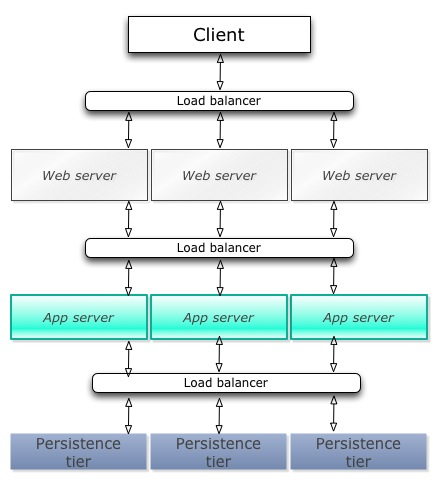
\includegraphics[width=10cm] {images/ntier2.jpg}}
	% Kommandoen \fbox tegner en ramme.
	\end{center}
	\caption{A distributed production architecture}\label{fig:ntier2}
	\end{figure}
				
				
\subsection{Examples of traditional web architectures}
In this section we will look at two examples of some common, traditional three-layered Web application architectures. The examples use Web application frameworks that is made for different programming languages, and promotes different architectural solutions. The purpose is to propose a set of popular web architectures, that will be used as a base to determine the architecture we use to design the first prototype in this project. 
				
\paragraph{MVC with Ruby on Rails}. The Rails framework for Ruby has become a highly popular backend technology for web applications with big commercial users like Twitter and Git-Hub \cite{railsPop}. The framework is built around the MVC design pattern \cite{mvc}. In a Rails application, the controllers act as thin classes that receives a Url request, and  delegates business logic to the Models. A Model is a Ruby class that implements the Domain Model design pattern, meaning it represents a particular domain resource in the application (for example a Movie, a User, a Book order etc), and it has all the business logic operations that are relevant for that particular resource. The Model objects also knows how to do database mapping, by communicating with for instance a relational database. The view layer consists of template files written in a template language like HAML\cite{haml} or ERB. These templates can reference data variables in a Model class, and are rendered into HTML files on the server before they are sent to the client's browser. 
				
Ruby on Rails encourages developers to use RESTful URL's so that these are automatically mapped to specific controller actions. The Rails developer can define the set of (RESTful) URL's that the application will support, and the framework will in return automatically create controller handlers for each URL with appropriate model objects that are being referred to in the URL. This principle is called \textit{convention over configuration}, because the framework sees the RESTful convention in the URL where a Model is referenced by a URI, and the operation is defined by either one of the HTTP methods GET, PUT, POST or DELETE. The controller actions usually calls a particular CRUD operation on a Model object that is referenced in the URL.  This is again accomplished automatically in Rails by using the convention over configuration principle. This is applied to the data source layer, where database tables are automatically created given the structure of a Model class, meaning that table names and attributes are created by default, determined by the names and types in the Model's ruby class. For instance, if a Model class is named \emph{Movie}, Rails will create a database table called \emph{Movies} that has all the fields that exists in the Movie class. 

The data source layer in Rails is typically built with the \textbf{Active Record design pattern}. This works by letting the Model objects implement CRUD operations for manipulating the database. This way, every Model class contains business logic operations (e.g validation, and business rules) and the functions requires to persist and manipulate the particular Model in the database.

The Rails framework makes it possible to build web applications quickly with a small amount of code, because Rails generates many of the basic structures and operations previously mentioned. In addition,
the loose coupling that results from the MVC pattern makes the application easy to distribute in a cloud environment, because if designed properly, each tier has a shared-nothing relationship. They are independent, and can be cloned and deployed on separate servers, as depicted in figure \vref{fig:ntier2}. This is much of the reason that Rails has gained a lot of popularity lately in the Web application industry \cite{someREF}% NEED REF!

\paragraph{Front Controller with SpringMVC}
SpringMVC is a web framework that wraps the Java Servlet API technology. The Java Servlet API are a set of classes that implements low-level protocols to communicate on the web (e.g HTTP). For example, the Java Servlet API implements an interface called \textit{javax.servlet.http.HttpSession}, which provides session management. This session implementation puts an Id (Called the JSESSIONID) in the User's Http cookie. This Id  refers a particular HttpSession object that belongs to the User, and it is maintained by Spring on the server. If the User does not allow cookies, Spring will instead rewrite every Url in the App to contain the JSESSIONID. The HttpSession objects can also be set to have a time-out value, in order to avoid wasting too much memory on the server. Also, The HttpSession object maintains an object container, such that the developer of SpringMVC Web apps can use this container to store state information. 

Just like with Rails, SpringMVC is also built around the MVC pattern. However, the framework also applies an architectural pattern called the Front Controller pattern. This pattern works by having one central servlet (the front controller) that receives all Http requests, and delegates control to an appropriate component that processes the request. This can be seen in figure \vref{fig:springmvc}.
				\begin{figure}
	\begin{center}
	\fbox{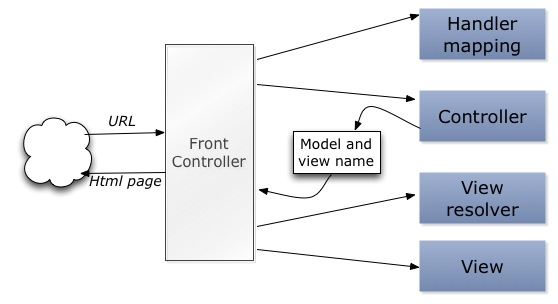
\includegraphics[width=10cm] {images/springmvc.jpg}}
	% Kommandoen \fbox tegner en ramme.
	\end{center}
	\caption{A request flow with spring MVC}\label{fig:springmvc}
	\end{figure}
	
When a request comes in, the front controller will ask a \textbf{handler mapper} to get a reference to a specific \textbf{controller} based on information provided in the request URL. A controller is a SpringMVC component (related to the Controller in the Model-View-Controller pattern) that is responsible for processing the actual requests. The handler mapper, is another Spring component that in addition to knowing what controller to issue based on a URL, performs pre- and post processing procedures, like validating the input from an HTML form, or marshaling an XML object to a Java class. When the handler mapper is finished pre-processing a URL request, it returns a reference to the controller that is meant to process the request. The front controller then delegates the request to this controller. The controller is usually responsible for performing some business operation implemented by the application programmer. When the business operation completes, the controller handler populates a \emph{model} object with necessary data that is to be displayed in the \textbf{view}. The model object is a simple key-value data structure that lets the developer easily reference its data from the view file. The controller function also returns the name for the view that is to be rendered together with the Model object. The \textbf{view} is a template file written in a template language like JSP or Velocity. It is the \textbf{view resolver} that maps a logical view name (e.g "homePageView") to a physical view name (e.g "/WEB-INF/views/homePageView.jsp"). Finally the view and the Model object is rendered to HTML and send back to the client. 
	
With Spring comes a great implementation of an inversion of control container (IOC)\cite {ioc}. Inversion Of Control is a programming methodology where the concrete types of object references are not know at compile time, because the references are instantiated and populated  by an assembler at run time. This avoids having tight couplings between classes, and promotes a flexible codebase. The IOC container is a module that is responsible for creating objects, populate their references  to other objects, and manage their complete lifecycle. The container is fully configurable, which makes it easy to decide how the classes are instantiated. For example, objects can be configured to be lazily instantiated, meaning the object won't be instantiated until it's first referenced. Also, there are multiple ways Spring's IOC container can be configured to create objects. In Spring, this is referred to as the object's \textbf{scope}. Some common scope-alternative are:

\begin{itemize}
\item{} Request - one instance is created for each HTTP request
\item{} Session - one instance is created for each Http session
\item{} Singleton - only one instance of the given class is created.
\end{itemize}

The IOC container provides a component based structure for the application by following the dependency inversion principle \cite {dip}. This principle states that objects should not depend upon details, but rather abstractions. This means that the spring IOC container will inject concrete objects into components (which are interface references and not references to concrete classes) at run time. This enhances the decoupling of classes, because they have the freedom to decide the types of their owning references at run time, instead of compile time. The container works as an object factory, and makes it easy to add new components to the application while at the same time hiding the implementation details of the added behavior. An alternative way of composing the application with external modules is to use the service locator design pattern \cite {j2ee}, which is a common approach taken in Java EE based applications. Dhrubojoyoti Kayal \cite{Kayal} shows how the service locator pattern can be implemented in Java Spring applications. However considering Spring already has an IOC implementation, it might lead to a lot of boilerplate code to assemble components using the Service locator pattern. 
			
Another nice feature with Spring is that it has built in support for both relational- and noSQL database management implementations, as well as transaction management. On top of this it supports annotation-based declarations making it easy to customize features using java annotations \footnote{Annotations: A way to add meta-data information in the source code. Metadata is often provided by configuration files, but annotations enables this information to be populated directly on the java declarations in the class files. An example is to use annotations to define how each variable in a java class is represented as a SQL column.} This conforms to the convention over configuration principle, which leads to simple and quick web application development. 
			
A typical domain logic layer in a Spring application is built with the service layer pattern \cite{serviceLayer}. In the service layer pattern, the business logic is split into two. A service layer that exposes an API that encapsulates all the business operations, and the domain model which structures the application's domain into nouns, typically represented as separate classes. The API, or service layer is categorized into logical abstractions called \textbf{services}, where each abstraction is hidden behind a facade \cite{facade}. A facade is an interface that contains simple access methods to a more complex set of data structures, like complex business operations or database access methods.  Hence, each service encapsulates complex business operations and communicates with lower layer data source functions. The domain objects typically has no logical functions, only private data attributes with accessor methods. The service classes communicates with the data source layer. The service classes are also responsible for handling transaction management, so that if a transaction fails, the service classes knows how to handle it. When performing transactions, the service classes delegates to the data source layer which would know how to communicate with the database and perform object-relational mapping. This could be done by implementing a customized object-relation mapping scheme, for instance by implementing the data mapper pattern described earlier, or by using an ORM tool like Hibernate or JPA. The latter case is similar to the active record pattern used in Ruby on Rails. Spring is one of the most popular frameworks for Java, as of 27th February 2013.\cite{springPopular}

TODO: Discuss front-controller vs MVC vs other shiet like page controller in php, template view.
\paragraph{Other examples}
Another popular architecture for thick-client Web apps is the \textbf{Page controller} pattern which is a commonly used with the Sinatra Web framework for Ruby. In this pattern, there is a strict relationship between a web page and a controller. Every (HTML) page on the app has a dedicated controller, such that the controller knows how to handle requests for the page it is responsible for, and it knows how to generate that page given the result of the request that is performed on that page. 

\section{Modern Web Application Architecture}
The motivation for proposing a reference model for modern Web app architecture has its roots in an architectural shift that started around 2008-2009.\cite{hales64} At this time, a new form of client-server interatcion scheme was emerging away from the traditional hyperlink/form-oriented request-response scheme, where each time the client interacts with the application, a request is sent to the server in which a new HTML page is created and sent back, and the browser has to reload the entire page. In addition, AJAX technology had been around for a long time, which usually was being used when some data is needed from the server for some minor interactive behavior. Building applications completely based on JavaScrip with Ajax for server communication was possible, however most developers had acknowledged the fact that such front-end oriented architectures doesn't scale in terms of code flexibility; it often ends up as piles of spaghetti code. This is partly because of web developers' relationship to JavaScript; as stated earlier, JavaScript has had its buggy features and lots of browser incompatibility problems since its early beginnings. Also, many professional developers has a misunderstood relationship to the language; they are not aware of JavaScript's key language features like object-orientation including prototypal inheritance, and functional- and dynamic programming facilities, having closures and a dynamic typing system. Also, developing large-scale JavaScript applications is difficult, because the language lacks constructs that facilitates flexible and modular code. It is possible to create namespaces and class-based structures with JavaScript, but it requires a lot of effort because it needs to be built from the ground up in every application. However, this was only until recent years, because a lot of work has been done to build frameworks that neatly solves these problems. 

%(TODO: skriv om n�r ECMAScript ble standardisert i kmap1), 
\subsection{Motivation}
The architectural shift began in 2010, when browser's capabilities to execute JavaScript increased tremendously. This was by the time when Google launched its Chrome browser with the powerful V8 JavaScript engine, and the compelling browsers followed along with similar JavaScript capabilities. Also, The JavaScript language itself has started to get much more endorsement from the web community with the standardization of ECMAScript, and Google's provenly working large-scale JavaScript applications like Gmail, Google Maps and also Node. This has led to many new experimental web architectures that takes a distance from the thick server model, and where application state is gradually moving from the server and into the client. However, not only is the application state moved to client, but also the application logic. This means that the core application moves from the backend to the client, leaving the backend being a simple and agnostic storage center for persisting the domain data in the application. Not only is this feasibly, but it's becoming increasingly popular. 

\subsection{The Idea}
Handling state on the client means that the one-to-one mappings between user interactions and controller handlers on the server are gone. Form requests and hyperlinks aren't sent directly to the backend, but instead handled on the front end. The client only contacts the server when domain data is needed to be fetched or manipulated in the database, authentication of users, or the browser needs to fetch static content like for instance images, movies, stylesheets or script files. In Reference Model 2.0, we propose an architecture where most of the responsibilities in a Web app is moved from the server to the client. These responsibilities include:
\begin{itemize}
\item{} Routing between pages
\item{} Render views into HTML
\item{} Sessions and state handling
\item{} Business logic operations
\item{} Input validation
\item{} Language translation of content
\item{} Deciding what to store in the database and when
\end{itemize}
 
Now, there are variations in how many of these responsibilities that are performed mainly by the client. Input validation for instance usually needs to be done on the server in addition to client-side validation, in case the user manages to contact the server directly without going through the front- end. Also, some applications might prefer to let the server be involved in routing between pages \cite{airbnbnode}, and perform some of the page rendering (ref to twitter). There are many good reasons for moving the backend responsibility to the client's front end. Some key advantages are:
	
	\begin{itemize}
	\item Centralization of the application's codebase, since much of the application logic, and the dynamic presentation logic is now located in the same place, and implemented in the same programming language
	 \item Less load on the server because more processing is moved to the client
	\item Facilitates smart front-end techniques like lazy loading of HTML- and script files, because JavaScript techniques can be used to only fetch HTML and script files when needed.
	\item The presentation logic and application logic lies much closer together in terms of source code. This facilitate tight cooperation and integration and be built with familiar design patterns in only one language: JavaScript. Such tight cooperation where hard to implement with the traditional approach, because it required tight cooperation between a template language (e.g JSP), JavaScript, and a backend language like Java.  
	\item Enables the server to offer a more general-purpose interface to the outside world. It no longed serves to deliver content to one particular client, but also other types of clients like third-party applications
\end{itemize}

\subsection{The Backend}
The responsibility of the backend is mainly to manage the database. It's interface is still exposed as controller handlers, however these are not customized for particular HTML form requests or hyperlinks that leads to a new HTML page. Instead, the backend exposes an \textbf{API} for interacting with the application's domain data. This API contains a set of public functions where each function is identified by a specific URL. Each URL refers to a domain entity in the application, and an operation that the server is to perform on the domain object. Note that this operation is usually not a complex business operation, but merely a single database operation. The operations offered by the backend API are commonly expressed using merely HTTP methods. Hence, the server API is a RESTfull service that adheres to the principles in the REST design pattern. Now, instead of creating and returning a complete HTML page upon each client request, the server would return a more fine-grained data object represented in a uniform data format like XML or JSON. This is a much more general-purpose solution, because external clients like mobile applications and other third party applications can now use the service offered by the application, because the service will no longer only respond with entire HTML pages, but a fine-grained format that is easier to manipulate and use as desired. This is often referred to as a service-oriented architecture \footnote{Many service-oriented architecture experts does not consider REST as a part of the SOA-paradigm, mainly because it is resource-oriented rather then service oriented}. 


\subsection{Front-end Frameworks}
Another interesting aspect of modern web application development is the evolution of JavaScript development environments. Not only has JavaScript been judged for being a language with many limitations, but it has also lacked proper development tools  like editors and debuggers, and frameworks for syntactic sugaring. Even though JavaScript is, and has always been a highly popular language for web applications, it has mostly been used as a tool to add dynamic behavior, input validation and simple Ajax calls to the server. With the increasing interest for large-scale JavaScript client applications, a huge amount of frameworks and language variations have been built. This includes:
\begin{itemize}
\item{} A huge amount of frameworks for structuring and organizing JavaScript code. \footnote{There is an project (REF) on www.Github.com(REF) where open source developers are implementing the same web application with different JavaScript frameworks to help developers choose a proper code organization framework for their web apps. (REF) }
\item{} Programming languages that compiles to JavaScript, to facilitate the development of large-scale JavaScript applications with a language that is more similar to traditional languages like Java or Ruby. Examples are Coffescript (ref) and clojure script(ref).
\item{} Syntactic sugaring frameworks that provides utility functions for operating on various JavaScript data structures, doing mathematical operations, or fixing browser compatibility issues.
\item{} Rendering engines for the front end, built to render HTML code with data objects.
\end{itemize}

	
\subsection{The Database}
Together with this thick-client approach one has also seen a sudden interest in alternatives to the traditional relational database. With the increasing popularity of applications being deployed and run in the cloud, there is a need to be able to distribute an application's database over many servers. Now it so happens that normal relational database structures has showed to have transactional challenges, and lacks scalability when distributed in the cloud \cite{dataCloud}. These issues, together with the demand for extreme high performance, has led to the development of new persistence technologies that are specifically designed to be replicated over multiple distributed database servers. The so-called noSQL paradigm is a common term for classification of database technologies that does not belong to the family of relational databases. In addition to being optimized for distribution, many noSQL database have addressed a flexible schema structure, or even not using schema's at all. This is in favor for the ability to customize entities in highly flexible manners, that would suit the application, unlike SQL which favors schema design that fits the entities and their relations.

Many noSql database have gained massive popularity in the last couple of years, because they has showed to deliver excellent performance and scalability, and because they sometimes fit more to the application's data needs. 

In the next few sections, I will dig further into the ideas and technologies that typically makes up the modern web-app architecture.
	
\subsection{Thick client tier}
In the traditional architecture, almost all of the business logic is implemented on the server, and the only code that is executed on the client is the JavaScript functions necessary for generating dynamic behavior in the browser. The idea in this proposition however, is to move the application's logic to the front-end. The business logic involves the domain objects and the operations that are performed on them, data validation, language translation of data, and communication with third-party API's. Instead of programming this logic in a proper backend language like Java or Ruby, this is  implemented in JavaScript, or a language that compiles to JavaScript, like CoffeeScript or Clojure script. The front-end source code is located on the web server as publicly available static assets. All the source code has its root in the main HTML file which is sent the client the first time he uses the app. The HTML file contains references to the JavaScript source file(s) that makes up the front-end application, such that the browser automatically fetches these when the main HTML page is being rendered. Typically the JavaScript code is separated over multiple source files. Also, the HTML page will have references to external JavaScript framework files that are not developed by the application programmer, but is used inside the app's own JavaScript code.
	
	The JavaScript code can either be sent to the client all at once when the web application is first accessed, or it can be lazily fetched. The latter means that the client will only ask for the necessary part of the code, when it needs it. This requires the source code to be split into separate code files so they can be sent individually from the server. This might be a performance benefit in case the whole JavaScript codebase is very big. A pitfall however might be that very many small JavaScript files are required at the same time. In some cases the TCP connection overhead might lead to a performance bottleneck because the browser usually creates a new TCP connection every time the browser requests something from the server. Sending all the scripts (and HTML and CSS files)  on startup gives the advantage of being able to gather all the JavaScript logic into one single file that can be extensively minimized and compressed. In this case, no further source files are needed to be fetched from the server, but the initial load time might be overwhelming. It is also possible to do a compromise, where the programmer gathers the most commonly used scripts into one compressed file that is sent initially, and then lets the client fetch the rest only when it is first needed. 
	
\subsection{Single-page Web Application Architecture}
One essential advantage of the thick client architecture is that server requests can now be limited. In the traditional approach, each user interaction with the page leads to a server requests that result in a new page, and the browser has to reload the whole page. This causes a disruption in the user experience. With the modern approach, the request goes straight to JavaScript event handlers. This way, the client stays on the same page during the whole session, requiring no new page reloads. If for instance a link in the navigation bar that leads to a different "section" in the app is requested, everything is done in the browser by manipulating the DOM tree so that the page moves to a new state. This leads could to a much more fluid user experience, because server requests can be avoided, and the browser does not have to reload the entire page. This principle is commonly referred to as a Single-page app (REF).  

If the front-end needs to synchronize data with the database it will send an asynchronous to the server. This could for instance be to save some data, or get some new data that needs to be displayed on the page. The client can also save data in the browser's memory, such that the more domain objects stored in the browser's JavaScript memory heap, the less requests has to be sent to the server. Depending on the application, write, update and delete operations will always sooner or later have to lead to a server request. In applications that requires all updated data to be available as close to real-time as possible, the operations has to be directly written to the database, in effect work as a write-through cache. In applications where this requirement is more relaxed, the front-end can choose to perform the server persistence at a later, more appropriate time. For web 2.0 applications, the former is often wanted, because users usually want to be see the latest updated data at all time. 
		
\subsection{REST API's and JSON}
The thick client model avoids letting the user communicate synchronously with the server. Instead, the JavaScript application that runs in the browser is responsible for knowing when it needs to communicate with the server. This would be whenever some domain objects that are not already in the browser's heap are requested, or some domain object must be persisted to the database. The requests to the server are exclusively done through a RESTful API. This means that all domain objects that are to be offered by the server, must be accessed through one of the HTTP methods \textit{GET, POST, PUT, or DELETE}. An example of a RESTful API that offers functions for persisting a Shredder object is showed in table below. A shredder is a guitarist in the web-app prototype that has been created in this thesis.
	
	\begin{center}
	\begin{tabularx}
	{\linewidth}{ |X|X|X| }
	    \hline
	    \textbf{Method} & \textbf{URL}  & \textbf{Description} \\ \hline
	    Get & www.shredhub.com/ shredder/1234 & Get shredder with id 1234 \\ \hline
	    Post & www.shredhub.com/ shredder/ ?name=Jude Swayer & Add shredder with name Jude Swayer  \\ \hline
	    Put & www.shredhub.com/ shredder/ 1234?country=Sweden & Update shredder with id = 1234 set country = Sweden \\ \hline
	    Delete & www.shredhub.com/ shredder/1234 & Delete shredder with id 1234 \\ \hline
	    \end{tabularx}
	    \end{center}
	    
	The server would respond with the domain objects in JSON format, instead of a complete HTML file. In effect, the return value is much more fine-grained. Also, the API is very consistent, because it adheres to a common interaction scheme, namely the HTTP functions Get, Post Put, and Delete. This creates a familiar and easily-to-understand server API. Many modern web application frameworks like Ruby on Rails, Spring MVC and Django are built based on the principles of REST, and will automatically create RESTfull controller functions based on the application's domain objects. This programming interface works really well with the thick client model, because now the client tier can be 100\% responsible of maintaining the application's state, and use the backend as a simple persistence API to store and deliver the domain objects. Hence, the backend is just a simple service that knows nothing about how to visualize the domain objects in HTML, leaving this responsible to the client tier. 
	
Modern REST API's very often use JSON as the transmission format. The reason is that it fits well into the programming model both on the front end and backend, because considering that the front end code is implemented in JavaScript, and JSON is part of the JavaScript language, it is very appropriate to use JSON as a transmission format because no marshaling has to be done on the client. At the same time on the backend, it is so that some of the noSQL technologies uses JSON objects, or JSON-similar syntax for persisting data. Hence we get a common transmission format that can be used across the whole software layer stack. 


	
\subsection{Modular JavaScript}

TODO: rewrite this:``''
How are pieces of JavaScript code defined today?
Defined via an immediately executed factory function.
References to dependencies are done via global variable names that were loaded via an HTML script tag.
The dependencies are very weakly stated: the developer needs to know the right dependency order. For instance, The file containing Backbone cannot come before the jQuery tag.
It requires extra tooling to substitute a set of script tags into one tag for optimized deployment.
This can be difficult to manage on large projects, particularly as scripts start to have many dependencies in a way that may overlap and nest. Hand-writing script tags is not very scalable, and it leaves out the capability to load scripts on demand.``''





A modular codebase is made up of highly decoupled, encapsulated pieces of coherent features that are implemented in separate modules. A codebase that consists of loosely coupled modules,  facilities a flexible and maintainable system, because the codebase contains less dependencies\cite{henrik}. This makes it easier to change one part of the system without harming any other.  
	As previously stated, the JavaScript programming language does not have module features built into the language. This means that it is up to the developers themselves to develop some sort of module framework. Various design patterns have been proposed to establish standard ways of developing modules, like the module and sandbox pattern \cite{jspatterns}. A lot of work has been done to provide open solutions for JavaScript developers to build modular JavaScript code, the two most famous being AMD (Asynchronous Module Definition) and CommonJS. Having the JavaScript code separated into modules means that these modules can be split into separate source files. That is what facilitates the lazy loading of JavaScript files previously mentioned. The modules can even depend on HTML files, so that whenever a JavaScript module is loaded, the HTML page will be loaded as well, and will be available as a text string inside the JavaScript module. With this feature, we can now state that the JavaScript modules are the first-class citizens in the application and hence decide which and when a given HTML page is to be displayed in the browser. This is an important difference from Reference-model 1.0 where the HTML pages where the first-class citizens, and the JavaScript code was just embedded inside the HTML. 
	
	The AMD principle was made to have a better alternative to loading scripts then the traditional group of \textit{<script>} tags embedded in HTML files. AMD brings an API that facilitates the separation of JavaScript into modules and defines the modules' dependencies to other modules. These dependencies are asynchronously loaded into the module, which avoids browsers having to block while waiting for synchronous module loading. the AMD API comes with two functions: require() and define(). Define() is used to encapsulate a JavaScript module while at the same time define the other module it depends on. The require() is used to asynchronously load modules into a function, in which the function will not be called until all the modules are loaded and ready to be used inside the function.

	%CommonJS is another module format meant to encapsulate JavaScrip into separate modules. %[MORE ON THIS].

	\subsection{Client side page-rendering}
	In Reference-model 1.0, every HTML page is completely rendered on the server and never changed after the page is sent to the clients. In Reference-model 2.0 however, this idea is completely abandoned. HTML pages are rendered "on the fly" with JavaScript code that is executed on the client side. The HTML pages contains templating markup that is detected by a JavaScript rendering engine. Whenever a new HTML page is to be loaded, or embedded into the current HTML page, a certain JavaScript function will be called. This function is responsible for asking the rendering engine to take an HTML page together with a set of JavaScript objects that represents the data that is to be displayed in the page, and finally return the HTML page with the JavaScript data rendered inside it. 
	As previously mentioned, the AMD model makes is possible to have JavaScript modules that depends on HTML files. This facilitates a nice programming model, because if the HTML pages are also separated into small, independent modules, then these modules can be stitched together to form complete HTML pages. For example, a JavaScript module might depend on a small HTML module, and when the JavaScript module is loaded, it can render the HTML module and insert it in the current HTML page. As such, HTML modules can be reused, removed or swapped out from the current HTML page by the JavaScript renderer. This enables a highly flexible way of altering contents of the HTML page, and also to easily glue together reusable front end solutions. 
		
	\subsection{Client state}
	Another part of Reference-model 2.0 is how the state is being kept between requests. The major goal of Reference-model 2.0 is to move much of the application logic from the server to the client. Hence, being able to keep the state client side is of high priority. In this architecture, we propose a solution to this by using HTML 5's Web Storage. The HTML 5 web storage is a standardization made by W3C that defines how to store structured data in the browser between page requests. It is supported in all modern browsers. HTML 5 web storage contains two storage containers: \textbf{localStorage} and \textbf{sessionStorage}. The difference is that local storage is being persisted even when the browser is closed, and it has no expiration date. The session storage is only kept in the browsers memory until the session is over, which means either if the user closes the tab or the browser. The storage enables developers to store lots of more data then what it supported with cookies. As an example, Internet Explorer 8 allows for sessionStorage up to 10 mega bytes, while a cookie is limited to 4 kilo bytes. The sessionSstorage is consists of a key-value data structure that is accessed by a simple JavaScript API.
	
	The session implementation is built by letting a JavaScript object be created when the web application is first accessed by the client user. The object is populated with account information for the user, and can be extended with data values that is appropriate to be cached in the browser. Each time the client tier changes state or receives some state information from the server, it can be persisted in the session object. Hence the server does not have to maintain a session object in memory for each user that is currently logged in to the web application.
	
\subsection{Node Js}
Node Js is a Web application framework built for using JavaScript as the programming language. This is one of the first (and most popular) solutions for developing JavaScript Web applications on the server. It runs in Google's V8 JavaScript engine. A big advantage this framework has compared to other frameworks like Rails and Spring, is that it is event-driven. This is a completely asynchronous programming environment that is centered around events, where clients subscribe to events are notified when the events are triggered. This avoids the blocking scenario that might occur in regular synchronous systems. It is completely possible use Node Js as the web application framework for Reference Model 1.0, the reason I mention it here is; because the backend is built with JavaScript when choosing Node, the application as a whole fits more with the Reference Model 2.0 which uses JavaScript as the core language on the front end. Hence you get a complete and pure JavaScript developer environment, in effect making the application more coherent, and less separated into different parts (backend/front-end).


\section{The Solutions}
The two reference models just described are popular approaches to how developers design and implement modern, interactive web apps. In this thesis, our goal is to compare these two approaches, in order to find any potential drawbacks or especial advantages. Therefore, we have taken the main ideas these reference models and applied them in two different software architectures for a prototypical web app. The first solution is called Architecture 1.0, while the latter is called Architecture 2.0. 

Architecture 1.0 is a thin client/thick server application. The backend is centered around a three-layered software architecture. This means that all the view logic happens in the presentation layer on the server, business logic operations happens in the domain logic layer, state is being kept on the server using Http sessions, and the front-end tier is tightly coupled to the server such that each Html form or link has a corresponding handler on the server which serves to generate a new Html page given the result of the request. The backend is build with Spring MVC, and is therefore a Java Web app. It uses a SQL database to persist data. 

Architecture 2.0, is a thick client/thin server architecture where control resides on the front end. State management, controller handling and business logic all happens on the front-end, which is built purely with JavaScript. The front-end is built with a sibling of the Model-View-Controller pattern, where the models are active record objects that uses the backend-server only as a simple data repository. The backend is offering its services through a Rest API, which is built with Node js. The Rest API manipulates the database, which is built with MongoDB. 
				
\section{Summary} 
TODO: Rewrite this
In this chapter we have proposed two very different web architectures. A short comparison of these two can be seen in the table below. The table sums up the major differences between the two architectures, where each row is concerning similar application issues. 

\begin{center}
	\begin{tabularx}
	{\linewidth}{ |X|X | }
	    \hline
	    \textbf{Reference-model 1.0} & \textbf{Reference-model 2.0} \\ \hline
	    Server-side page rendering & Client-side page rendering \\ \hline
	    Application logic runs on server (thick server) & Application logic runs in browser (thick client)  \\ \hline
	    Session state stored on server & Session state stored in browser \\ \hline
	    Form-based interaction with complete html pages returned & RESTfull ajax requests for JSON objects and asynchronous module loading \\ \hline
	    Relational database system & Document-oriented database based on key-value semantics \\ \hline
	    \end{tabularx}
	    \end{center}


Reference-model 1.0 had a thin client model with all the business logic performed on the server. The server's job was to perform the business operations, execute database operations and create and render a view that is sent back to the client. I argued that having a decoupled three-tier architecture could make it possible to distribute each tier in the cloud, but the problem with having a relational database could lead to that being a bottleneck. The latter approach had a thick client model where most of the logic was performed in the client's browser (I.e front-end), primarily using the server for database operations. This could lead to a structured and loosely coupled front-end implementation, as well as a reduced amount of data sent back and forth between the client and server. The RESTfull architecture, together with asynchronous HTML/JavaScript loading can make it possible to limit the data that is sent back back from and to the server, since the only time a complete Html page request is required is the first time the page is accessed. However the first HTTP request might turn in to being a very big data package, since a lot of JavaScript has to be sent to the client.
This could in worst case could lead to a very slow initialization time.  Also because the data format is cross-platform, other external clients like third party users and mobile applications can use the service offered by the application. Finally, the noSQL database characteristics seems to be more suitable in a cloud environment, because it is possible to shard the database tier with in a shared-nothing manner. It also provides programmer friendliness due to its simple syntax. At the end of the chapter we stated that the two reference models discussed in this thesis are used as a base for designing and implementing the two architectures that have been built for this thesis. 
